
\begin{frame}
	\titre{Ingrédients}
	
	\begin{description}[labelindent=6pt,style=multiline,leftmargin=1.3in]
		 \setlength\itemsep{1.4em}
\pause
\item[Hein ?] On n'a pas caractérisé ce qu'on peut utiliser comme prémisse ou conclusion
\pause
\item[Exemple] \begin{tabular}{l}
Je\\
On mange à quelle heure ?\\ \cline{1-1}
serveur blond\\
\end{tabular}
\pause \newline
\item[Idée] On ne veut utiliser que des énoncés qui contiennent du sens 

\pause
\item[] C'est ce qu'on va appeler les \textbf{propositions}
	\end{description}
\end{frame}



\begin{frame}
	\titre{Proposition}
	
	\begin{description}[labelindent=6pt,style=multiline,leftmargin=1.3in]
		 \setlength\itemsep{1.4em}

\item[Intuitivement] Une expression que l'on peut considérer comme \textbf{vraie} ou \textbf{fausse}
\pause
\item[Techniquement] Une expression qui peut recevoir une \textbf{valeur de vérité} 
\pause
\item[Exemples] Il pleut \pause
%\item[] Jean-Paul a faim et Jean-Charles a soif \pause 
\item[] Si vous faites les exos hebdomadaires, vous aurez un bonus sur votre note finale \pause
%\item[] Brian de Palma est un réalisateur génial \pause
\end{description}
 Les hommes justes qui redoutent la puissance de Dieu n’endureront pas les
souffrances éternelles de l’enfer.
\end{frame}


\begin{frame}
	\titre{Les \textbf{non-}propositions}
	
	\begin{description}[labelindent=6pt,style=multiline,leftmargin=1.3in]
		 \setlength\itemsep{1.4em}

\item[`Petites` expressions] Je (référence)
\pause
\item[] Grand (prédicat) \pause
\item[] Actrice norvégienne (prédicat complexe) \pause
\item[] Manger bruyamment (id) \pause
\item[Interrogatives] A quelle heure on mange ? \pause
\item[Impératives] Ne me parle pas de Jean-Louis 
\end{description}
\end{frame}



\begin{frame}
	\titre{Classification des props.}
	Propositions complexes vs. simples \newline
	\pause
	
	\begin{description}[labelindent=6pt,style=multiline,leftmargin=1.3in]
		 \setlength\itemsep{1.4em}

\item[Complexe] contient d'autres propositions \pause
\item[Exemples] Jean-Charles a faim et Jean-Luc a soif\pause
\item[] Chloé est triste car son amie l'a abandonnée\pause
\item[Attention] Une prop. complexe ne \textit{porte} pas forcément \textbf{le sens} d'autres propositions \pause
\item[Exemple] Si je me réveille demain, j'irai en cours
%\item[Remarque] \only<7>{Brian de Palma est un réalisateur américain} \only<8>{Jules est un faux blond} \pause
\end{description}
\end{frame}


\begin{frame}
	\titre{Classification des props.}
	Propositions complexes vs. simples \newline

	
	\begin{description}[labelindent=6pt,style=multiline,leftmargin=1.3in]
		 \setlength\itemsep{1.4em}

\item[Remarque] Les props. complexes peuvent être piégeuses\footnote{Notamment vis-à-vis de la généralisation, ou systématisation, dont on a discuté la dernière fois}\pause
\item[Exemple] Brian de Palma est un réalisateur américain \pause
\newline $\Rightarrow$ Brian de Palma est américain \pause
\newline $\Rightarrow$ Brian de Palma est un réalisateur\pause
\item[vs.] Jules est un faux blond \pause
\newline $\not\Rightarrow$ Jules est blond \pause
\newline $\not\Rightarrow$ Jules est faux (??)

\end{description}
\end{frame}



\begin{frame}
	\titre{Classification des props.}
	Propositions complexes vs. simples \newline

	
	\begin{description}[labelindent=6pt,style=multiline,leftmargin=1.3in]
		 \setlength\itemsep{1.4em}

\item[Remarque] Une prop. peut être arbitrairement complexe \pause
% expliquer que la littérature est pas entièrement claire, mais à priori approche algèbrique
% de toute façon, OSEF au fond de Port-Royal, autant prendre des bons refléxes pour après
% dessin avec un simili-arbre-syntaxique
\item[Exemple] Si Alice apprend que Bob a dit à Charles que Diane en veut à Elsa parce qu'elle a dit du mal du dessin que Flavien lui a fait quand Georges est venu à l'anniversaire d'Hector, Inès sera triste. \pause
\item[Props. simples] Du coup, les propositions \textit{atomiques}

\end{description}
\end{frame}



\begin{frame}
\titre{Retour sur l'exemple}

La notion \underline{précise} de prop. complexe est très boiteuse (et on va d'ailleurs très vite s'en désintéresser)\newline \pause

La définition donnée est \textbf{externe}, dans le sens où elle nous aide à \textit{reconnaître} des propositions (trouvées n'importe où)\pause \newline

On trouve aussi dans la littérature une définition \textbf{interne}, c'est à dire qui décrit la \textit{construction} des propositions complexes, mais elle n'est pas très formelle (donc pas super satisfaisante).\newline \pause

En logique propositionnelle et du premier ordre, on aura une définition interne bien définie et carrée, qui du coup sera dure à appliquer en pratique (compromis auquel on aura du mal à échapper).

\end{frame}

%
%\begin{frame}
%	\titre{Retour sur l'exemple}
%	
%`Sous-propositions` de l'exemple
%	
%\begin{description}[labelindent=6pt,style=multiline,leftmargin=4in]
%\item[Inès sera triste]
%\end{description}
%
%\begin{description}[labelindent=6pt,style=multiline,leftmargin=4in]
%\item[Alice apprend que (...) à l'anniversaire d'Hector]
%\end{description}
%
%
%\begin{description}[labelindent=6pt,style=multiline,leftmargin=4in]
%\item[Bob a dit (...) à l'anniversaire d'Hector]
%\end{description}
%
%
%\begin{description}[labelindent=6pt,style=multiline,leftmargin=4in]
%\item[Diane en veut à (...) à l'anniversaire d'Hector]
%\end{description}
%
%\begin{description}[labelindent=6pt,style=multiline,leftmargin=4in]
%\item[Diane en veut à Elsa]
%\end{description}
%
%\begin{description}[labelindent=6pt,style=multiline,leftmargin=4in]
%\item[Elsa a dit du mal du dessin que Flavien lui a fait quand Georges est venu à l'anniversaire d'Hector]
%\end{description}
%
%
%\end{frame}
%
%
%\begin{frame}
%	\titre{Retour sur l'exemple}
%	
%\begin{description}[labelindent=6pt,style=multiline,leftmargin=4in]
%\item[Alice apprend]
%\end{description}
%\pause NON\pause, plusieurs versions du verbe `apprendre`\pause : `X apprend`\pause, `X apprend Y`\pause, `X apprend Y à Z`\pause, etc ?\pause
%
%
%\begin{description}[labelindent=6pt,style=multiline,leftmargin=4in]
%\item[Diane a dit du mal du dessin]
%\end{description}
%\pause NON\pause, sans le `que truc`, `le dessin` ne désigne plus (forcément) le même objet\pause, on a donc une proposition qui n'apparaît pas dans la phrase complète
%\pause
%\begin{description}[labelindent=6pt,style=multiline,leftmargin=4in]
%\item[Elsa a dit du mal]
%\end{description}
%\pause NON\pause, même raison\pause : en enlevant `du dessin`, on change complètement de proposition
%
%
%\end{frame}
%
%
%\begin{frame}
%	\titre{Retour sur l'exemple}
%	
%\begin{description}[labelindent=6pt,style=multiline,leftmargin=4in]
%\item[Flavien a fait un dessin à Diane quand Georges est venu à l'anniversaire d'Hector]
%\end{description} 
%\textcolor{white}{\_} \newline
%\begin{description}[labelindent=6pt,style=multiline,leftmargin=4in]
%\item[Georges est venu à l'anniversaire d'Hector]
%\end{description}
%\pause
%\begin{description}[labelindent=6pt,style=multiline,leftmargin=4in]
%\item[?]
%\end{description}
%
%\end{frame}
%
%
%\begin{frame}
%		\titre{Retour sur l'exemple}
%%	Si Alice apprend que Bob a dit à Charles que Diane en veut à Elsa parce qu'elle a dit du mal du dessin que Flavien lui a fait quand Georges est venu à l'anniversaire d'Hector, Inès sera triste. 
%	
%	\begin{tikzpicture}[scale=.53]
%
%\Tree[.{si \_ alors \_} [.{\_ apprend \_} Alice [.{\_ a dit \_ à \_} Bob [.{\_ parce que \_ } {Diane en veut à Elsa$_1$} [.{\_ a dit \_} elle$_1$ [.{du \_ de \_} mal [.{le \_ que \_ } dessin [.{\_ quand \_} {Flavien lui a fait} {\begin{tabular}{c}
%     Georges est venu  \\
%     à l'anniversaire d'Hector \\
%  \end{tabular}} ] ] ] ] ] Charles ] ] {Inés sera triste} ]
%\end{tikzpicture}
%
%	
%	\end{frame}


\begin{frame}
	\titre{Classification des props.}
	Propositions (simples) \textbf{catégoriques} vs. \textbf{thétiques} \newline
	
		\begin{description}[labelindent=6pt,style=multiline,leftmargin=1.3in]
		 \setlength\itemsep{1em}
\pause
\item[Def. classique] Une propostion est une expression comportant un sujet et un prédicat (une propriété)
\pause
\item[Exemple] \underline{Le petit chat} est \underline{mort}
\pause 
\item[] \underline{Jean-Louis} est un \underline{canard}
		 \item[] \textcolor{white}{ligne cachée}
		 \item[] \textcolor{white}{ligne cachée}

	\end{description}
\end{frame}


\begin{frame}
	\titre{Classification des props.}
	Propositions (simples) \textbf{catégoriques} vs. \textbf{thétiques} \newline
	
		\begin{description}[labelindent=6pt,style=multiline,leftmargin=1.3in]
		 \setlength\itemsep{1em}
\item[Sujet] Expression référentielle designant un individu (une entité $\in \cal U$) ou une classe d'indivus/entités \pause
\item[] $\Rightarrow$ \textbf{Ce dont on parle}\pause
\item[Prédicat] Propriété que l'on affirme de / que l'on attribue à un sujet \pause
\item[] Techniquement, c'est une fonction de vérité $\cal U \rightarrow \{V,F\}$ \pause
\item[] $\Rightarrow$ \textbf{Ce qu'on en dit}

	\end{description}
\end{frame}


\begin{frame}
	\titre{Classification des props.}
	Propositions (simples) \textbf{catégoriques} vs. \textbf{thétiques} \newline
	
		\begin{description}[labelindent=6pt,style=multiline,leftmargin=1.3in]
		 \setlength\itemsep{1em}
\item[Définition] Les propositions qui obéissent clairement à cette décomposition sont appelées (depuis Aristote) \textbf{jugements catégoriques} \pause
\item[Par contraste] les \textbf{jugements  thétiques} n'ont pas de sujet \textit{réel}\pause, même s'il peut y avoir un sujet grammatical \pause
\item[] Il faisait beau 
\item[] Il y a des fleurs
	\end{description}
\end{frame}



\begin{frame}
	\titre{Classification des props.}
	Propositions (simples) \textbf{catégoriques} vs. \textbf{thétiques} \newline
	
La notion est importante en syllogistique (on y revient), mais plus tard critiquée, notamment par Frege \pause \newline

De façon générale, les classes des propositions en syllogistiques sont peu élégantes et pas toujours très bien définies\pause \newline

Les formalismes plus mathématiques \textit{à la Frege} (ie. la logique propositionnelle) s'attaqueront à ce problème\pause \newline

Aujourd'hui, il est évident que la distinction props. catégoriques / thétiques est pas claire

\end{frame}



\begin{frame}
	\titre{Classification des props.}
	Propositions (simples et catégoriques) \textbf{singulières} vs. \textbf{quantifiées}\newline
	
		\begin{description}[labelindent=6pt,style=multiline,leftmargin=1.3in]
		 \setlength\itemsep{1em}
\item[Singulières] Les phrases ayant un sujet référentiel simple, \textbf{unique} et \textbf{identifié}\pause
\item[Exemple] Lapinot est gentil \pause
\item[] Mon voisin d'en face est photographe \pause
\item[] Le petit chat n'est (finalement) pas mort \pause
\item[] J'ai mal dormi
	\end{description}
\end{frame}

\begin{frame}
	\titre{Classification des props.}
	Propositions (simples et catégoriques) \textbf{singulières} vs. \textbf{quantifiées}\newline
	
		\begin{description}[labelindent=6pt,style=multiline,leftmargin=1.3in]
		 \setlength\itemsep{1em}
\item[Quantifiées] Sujet collectif \pause
\item[Exemple] Tous les élèves m'écoutent \pause
\item[] Quelques films magnifiques sont sortis cette année \pause
\item[] Personne n'a rien à cacher\pause
\item[Question] Le dernier exemple n'est pas très joli, est-ce qu'on peut en trouver une autre formulation (équivalente) ?
	\end{description}
\end{frame}


\begin{frame}
	\titre{Classification des props.}
	%Propositions \textbf{singulières} vs. \textbf{quantifiées}
	
		\begin{description}[labelindent=6pt,style=multiline,leftmargin=1.3in]
		 \setlength\itemsep{1em}
\item[Exemple] Personne n'a rien à cacher \pause $\equiv$ Tout le monde a quelque chose à cacher\pause
%\item[Remarque] Si vous avez du mal à le voir, remplacez `n'a rien à cacher` par `n'a rien dans la tête`\pause 
\item[Intuition] Comprendre la phrase comme `Pour toute personne $x$, il est faux que $x$ a \textbf{la propriété de n'avoir rien à cacher}`\pause
\item[$\equiv$]  `Pour toute personne $x$, \textbf{il est faux qu'il n'existe pas} $y$ que $x$ doit cacher`\pause
\item[$\equiv$] `Pour toute personne $x$, il existe $y$ que $x$ doit cacher` \pause $\equiv$ `Tout le monde a quelque chose à cacher`

	\end{description}
\end{frame}

\begin{frame}
	\titre{Classification des props. quantifiées}
	
		\begin{description}[labelindent=6pt,style=multiline,leftmargin=1.3in]
		 \setlength\itemsep{1em}
\item[Idée] On va essayer de raffiner la distinction de proposition quantifiée \pause en fonction de la `nature` de la quantification\pause
\item[Rappel des exemples] Tous les élèves m'écoutent 
\item[] Quelques films magnifiques sont sortis cette année
\item[] Personne n'a rien à cacher\pause
\item[Du coup] des idées ?
	\end{description}
\end{frame}



\begin{frame}
	\titre{Classification des props. quantifiées}
	Propositions \textbf{universelles}
	
		\begin{description}[labelindent=6pt,style=multiline,leftmargin=1.3in]
		 \setlength\itemsep{1em}
\item[En gros] Sujets introduits par `tous les`, `tout`, `chaque` \& cie\only<1-3>{\textcolor{white}{, mais aussi `nul`, `aucun`}}\only<4>{. Autre chose ?\textcolor{white}{oulouloulou}}\only<5->{, mais aussi `nul`, `aucun`}\pause
\item[Exemples] Tous les élèves m'écoutent\pause
\item[] Tout enfant a une friandise préférée\pause
\pause \pause
\item[] Personne n'a rien à cacher \pause
\item[] Nul n'est infaillible\pause
\item[] Aucun linguiste n'est cool
	\end{description}
\end{frame}


\begin{frame}
	\titre{Classification des props. quantifiées}
	Propositions \textbf{universelles}
	
		\begin{description}[labelindent=6pt,style=multiline,leftmargin=1.3in]
		 \setlength\itemsep{1em}
\item[En gros] `tous les`, `tout`, `chaque`, `nul`, `aucun`\pause, encore autre chose ?\pause
\item[Exemples] Un polar coréen, ça finit mal \pause
\item[] Le canard est un mammifère\pause
\item[A rajouter] les phrases introduites par des déterminants non intrinsèquement quantificationnels, mais prenant une valeur universelle\pause
\item[] C'est à dire les généralisations
	\end{description}
\end{frame}


\begin{frame}
	\titre{Classification des props. quantifiées}
	Propositions \textbf{universelles}
	
		\begin{description}[labelindent=6pt,style=multiline,leftmargin=1.3in]
		 \setlength\itemsep{1em}
\item[Intuition] Toute phrase qu'on peut transformer en `Tous les \textit{individus} qui ont la propriété X ont aussi la propriété Y`
\item[Remarque] On peut quantifier sur plusieurs propriétés\pause 
\item[] `Un polar coréen, ça finit mal` $\equiv$ `Tous les individus qui ont la propriété (\textit{complexe}, ou double) d'être des films coréens ont aussi la propriété de finir mal`\pause
\item[Exemple] `Tout film japonais ou pièce allemande classique me fait rire et pleurer`
	\end{description}
\end{frame}

\begin{frame}
	\titre{Classification des props. quantifiées}
	Propositions \textbf{universelles}
	
		\begin{description}[labelindent=6pt,style=multiline,leftmargin=1.3in]
		 \setlength\itemsep{1em}
\item[Exemples ?] Toutes les voitures volent\pause : yes \pause
\item[] Les poules volent \pause : yes \pause
\item[] Tous les allemands n'étaient pas cinéphiles\pause : nein ($\equiv$ `Il y a des allemands qui n'étaient pas cinéphiles`)\pause
\item[] Le joueur moyen de LoL est tendu\pause : yes\pause
\item[] Chaque journée est un enfer\pause : yes\pause
\item[] Tous mes amis ne sont pas fiables\pause : nein
	\end{description}
\end{frame}



\begin{frame}
	\titre{Classification des props. quantifiées}
	Propositions \textbf{particulières}
	
		\begin{description}[labelindent=6pt,style=multiline,leftmargin=1.3in]
		 \setlength\itemsep{1em}
\item[En gros] Propositions introduites par `un`, `certains`, `quelques` \& cie\pause
\item[Exemples] Certains éléphants ont une trompe\pause
\item[] Quelque malheur a dû arriver\pause
\item[] Quelques enfants ont explosé\pause
\item[] Un mec est passé hier soir\pause
\item[] Un poisson a peu de mémoire\pause : ça dépend \pause(mais à priori non)
	\end{description}
\end{frame}


\begin{frame}
	\titre{Classification des props. quantifiées}
	Attention : confusion \textbf{particulières} et \textbf{singulières} 
	
		\begin{description}[labelindent=6pt,style=multiline,leftmargin=1.3in]
		 \setlength\itemsep{1em}
\item[singulière] A propos d'un seul individu \textbf{précis}\pause
\item[Exemples] Jean-Louis a bien mangé\pause
\item[] \textbf{Ce} lapin a de petites oreilles\pause
\item[particulière] Parle d'un individu \textit{pas identifié}\pause
\item[Exemple] \textbf{Un} lapin (quelque part) a de petites oreilles
	\end{description}
\end{frame}

\begin{frame}
	\titre{Classification des props. quantifiées}
	Propositions \textbf{particulières}
	
		\begin{description}[labelindent=6pt,style=multiline,leftmargin=1.3in]
		 \setlength\itemsep{1em}

\item[Remarque] Certains éléphants ont une trompe
\item[] Quelque malheur a dû arriver
\item[] Quelques enfants ont explosé
\item[] Un mec est passé hier soir\pause
\item[Attention] Tous ces énoncés sont vrais s'il y a \textbf{au moins un} élément du sujet qui vérifie le prédicat \pause (désolé, c'est non-négociable)
	\end{description}
\end{frame}


\begin{frame}
	\titre{Classification des props. quantifiées}
	Propositions \textbf{particulières}
	
		\begin{description}[labelindent=6pt,style=multiline,leftmargin=1.3in]
		 \setlength\itemsep{1em}
\item[Rappel] Dans les universelles, on avait des \textbf{quantificateurs} \textbf{affirmatifs} (`tous les`, `tout`, `chaque`, `un`, `le`, etc) et \textbf{négatifs} (`nul`, `aucun`)\pause
\item[Remarque] On a aussi une notion de affirmatif/négatif pour les props particulières\pause, mais qui se fait cette fois au niveau du verbe\pause
\item[Exemples] Certaines banques n'ont pas été braquées
\item[] Au moins un prof n'est pas compétent 
	\end{description}
\end{frame}


\begin{frame}
	\titre{Classification des props. quantifiées}
	On peut donc distinguer 4 classes de propositions quantifiées en faisant intervenir les 2 paramètres \pause
			\begin{description}[labelindent=6pt,style=multiline,leftmargin=1.3in]
		 \setlength\itemsep{1em}
\item[A] Universelle affirmative 
\item[E] Universelle négative
\item[I] Particulière affirmative 
\item[O] Particulière négative\pause
\item[Question] Des trucs qui ont l'air de ne pas aller avec cette classification ?\pause
\item[] Toutes les props. ne sont pas couvertes (`La plupart des X sont Y`)
	\end{description}
	
\end{frame}



\begin{frame}
	\titre{Le dessin pour résumer}
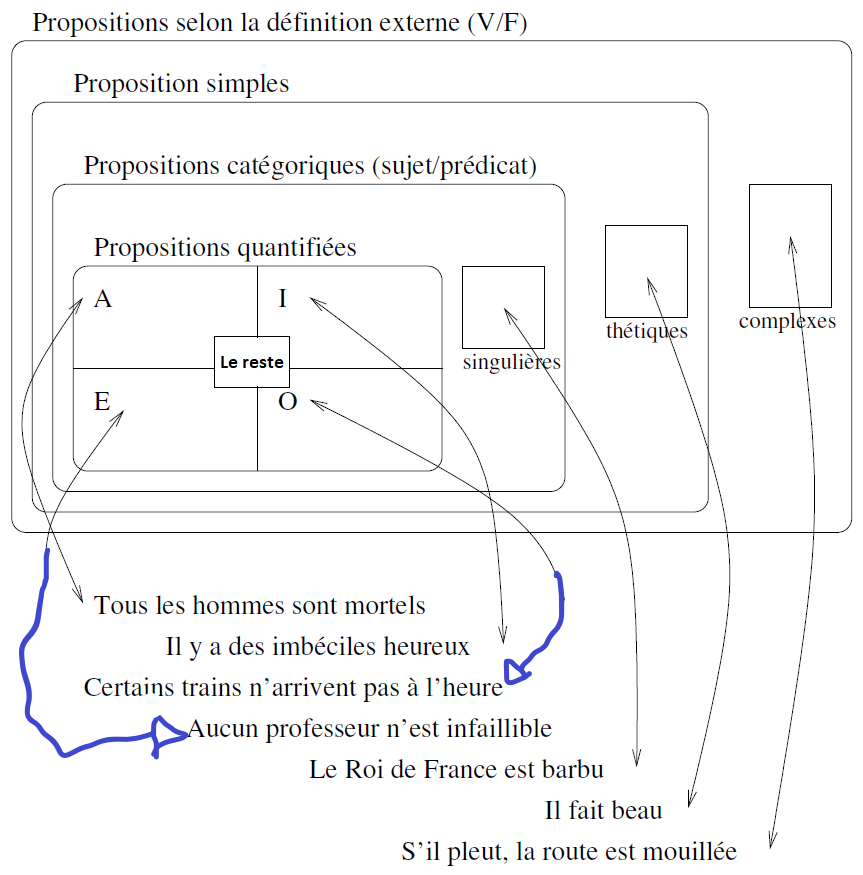
\includegraphics[scale=0.31]{syntheseProps.png}
\end{frame}




%---------------- intro -------------------

\begin{frame}
	\titre{Relations entre propositions}

			\begin{description}[labelindent=6pt,style=multiline,leftmargin=1.3in]
		 \setlength\itemsep{1em}
\item[Inverse \only<5->{?}] \textcolor{white}{lol} 
	 \pause
\item[Exemple] Tout prof est sympa\pause 
\item[] Quelle est la proposition \textit{inverse} ?\pause 
\item[] `Aucun prof n'est sympa` ?\pause 
\item[] Ca dépend de ce qu'on appelle l'\textit{inverse}\pause
\item[] On va distinguer les notions de propositions \textbf{contraires} et \textbf{contradictoires}
	\end{description}
	
\end{frame}



%------------------ Contraire ----------------------
\begin{frame}
	\titre{Relations entre propositions}

			\begin{description}[labelindent=6pt,style=multiline,leftmargin=1.3in]
		 \setlength\itemsep{1em}
\item[Contraires] P et Q sont contraires $\equiv$ elles ne peuvent pas être vraies en même temps 
	 \pause
%\item[En maths] $(P \rightarrow \neg Q) \wedge (Q \rightarrow \neg P)$\pause 
\item[En français] P et Q sont incompatibles\pause 
\item[Exemple] Proposition contraire de `Tout prof est sympa` ?\pause 
\item[] `Aucun prof n'est sympa` ? \pause Oui\pause
\item[] On peut en trouver d'autres ?\pause
\item[] `Il y a au moins un prof qui n'est pas sympa`
	\end{description}
\end{frame}



\begin{frame}
	\titre{Relations entre propositions}

			\begin{description}[labelindent=6pt,style=multiline,leftmargin=1.3in]
		 \setlength\itemsep{1em}
\item[Contraires] P et Q sont incompatibles
	 \pause
%\item[En maths] $(P \rightarrow \neg Q) \wedge (Q \rightarrow \neg P)$\pause 
\item[Exemple] Propositions contraires de `Le chat est mort et le chien est blond` ?\pause 
\item[] Le chat n'est pas mort \pause 
\item[] Le chien n'est pas blond\pause
\item[] Le chat n'est pas mort et le chien n'est pas blond\pause
\item[] Le chat n'est pas mort ou le chien n'est pas blond
	\end{description}
\end{frame}




%------------------------ Contradiction ----------------------------

\begin{frame}
	\titre{Relations entre propositions}

			\begin{description}[labelindent=6pt,style=multiline,leftmargin=1.3in]
		 \setlength\itemsep{1em}
\item[Contradiction] P et Q sont contradictoires si et seulement si elles ne peuvent être ni vraies ni fausses en même temps 
	 \pause
%\item[En maths] $(P \rightarrow \neg Q) \wedge (Q \rightarrow \neg P)$\pause 
\item[En français] On a toujours soit P, soit Q\pause 
\item[Exemple] Proposition contradictoire de `Tout prof est sympa` ?\pause 
\item[] `Il y a au moins un prof qui n'est pas sympa`\pause
\item[] Une autre ? \pause Non, pour toute proposition P, \textbf{unicité} de $\neg P$ (à reformulation près)
	\end{description}
\end{frame}



\begin{frame}
	\titre{Relations entre propositions}

			\begin{description}[labelindent=6pt,style=multiline,leftmargin=1.3in]
		 \setlength\itemsep{1em}
\item[Contradiction] On a toujours soit P, soit Q
	 \pause
%\item[En maths] $(P \rightarrow \neg Q) \wedge (Q \rightarrow \neg P)$\pause 
\item[Exemple] Le chat est mort et le chien est blond\pause 
\item[$\neg$] Le chat n'est pas mort ou le chien n'est pas blond\pause 
\item[Exemple] Certaines baleines sont sympathiques\pause
\item[$\neg$] Aucune baleine est sympathique \pause
\item[Exemple] Certains films français sont pas géniaux \pause
\item[$\neg$] Tous les films français sont géniaux 
	\end{description}
\end{frame}


\begin{frame}
	\titre{Relations entre propositions}

			\begin{description}[labelindent=6pt,style=multiline,leftmargin=1.3in]
		 \setlength\itemsep{1em}
\item[Contradiction] On a toujours soit P, soit Q
	 \pause
%\item[En maths] $(P \rightarrow \neg Q) \wedge (Q \rightarrow \neg P)$\pause 
\item[Exemple] Personne ne comprend ce cours \pause
\item[$\neg$] Quelqu'un comprend ce cours\pause
\item[Question] Vous avez remarqué quelque chose ?\pause
\item[] Quelque chose qui ressemblerait à une règle concernant les contradictions et les propositions quantifiées ?
	\end{description}
\end{frame}


\begin{frame}
	\titre{Relations entre propositions}

			\begin{description}[labelindent=6pt,style=multiline,leftmargin=1.3in]
		 \setlength\itemsep{1em}
\item[A] Tous les profs sont gentils
	 \pause
%\item[En maths] $(P \rightarrow \neg Q) \wedge (Q \rightarrow \neg P)$\pause 
\item[I] Quelques profs sont gentils\pause
\item[E] Aucun prof n'est gentil \pause
\item[O] Quelques profs ne sont pas gentils\pause
\item[Question] Que peut-on dire de chaque couple tiré dans cette liste de propositions ?\pause
\item[Indice] On va devoir introduire deux nouvelles relations (simples) entre propositions
	\end{description}
\end{frame}


\begin{frame}
	\titre{Le carré d'opposition}
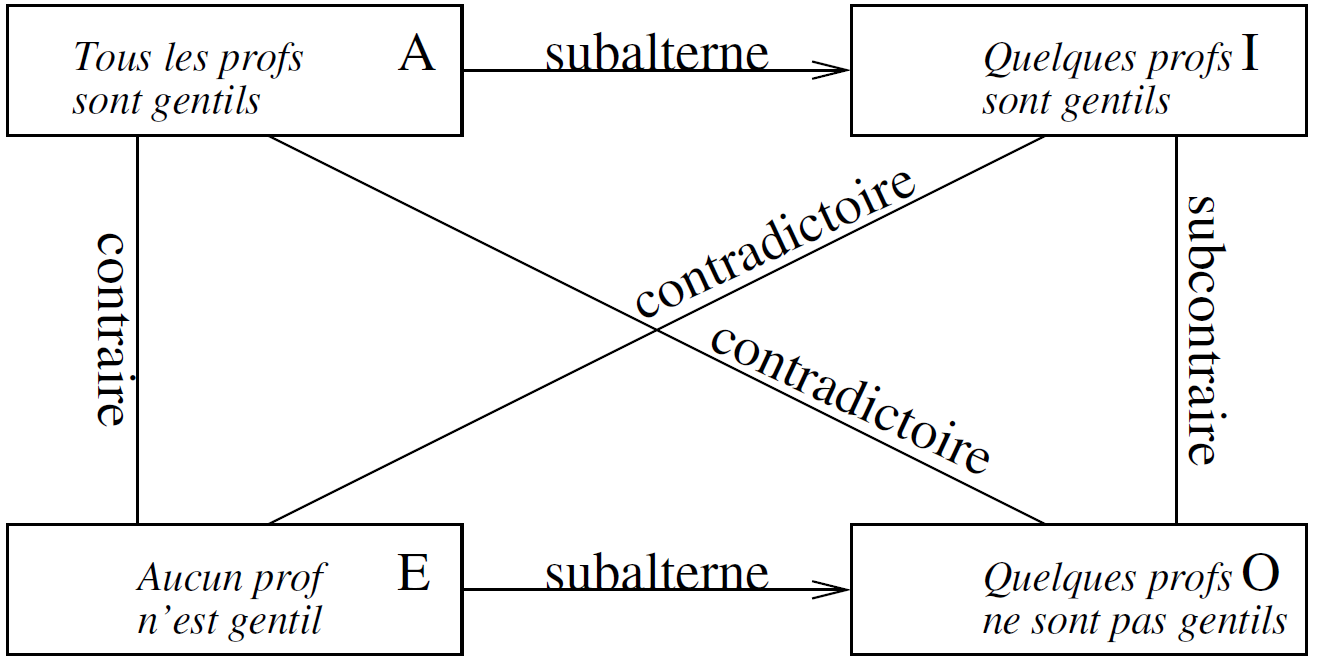
\includegraphics[scale=0.32]{carre.png}
\end{frame}


\begin{frame}
	\titre{Le carré d'opposition}

			\begin{description}[labelindent=6pt,style=multiline,leftmargin=1.3in]
		 \setlength\itemsep{1em}
\item[Subcontraire] P et Q sont subcontraires si elle ne peuvent pas être fausses en même temps\pause
\item[Remarque] I et O sont subcontraires, tandis que leurs contradictions (ou négations) sont contraires entre elles\pause
\item[] Coïncidence ? \pause Sans doute pas\pause
\item[Subalterne] P est subalterne de Q si Q implique P\pause, c'est à dire si chaque fois que Q est vraie, P l'est nécessairement aussi.
	 \pause
\item[def alternative] P est une version appauvrie (en information) de Q
	\end{description}
\end{frame}


\begin{frame}
	\titre{Le début du merdier}
			\begin{description}[labelindent=6pt,style=multiline,leftmargin=1.3in]
		 \setlength\itemsep{1em}
\item[Contraires] P et Q sont contraires $\equiv$ elles ne peuvent pas être vraies en même temps 
\item[Contradiction] On a toujours soit P, soit Q\pause
\item[Cependant] Pour les logiciens ... \pause c'est le contraire !\pause
\item[] Ils ont néanmoins plus l'habitude de dire `propositions inverses` que contraires \pause
\item[] On utilisera $P = \neg Q$ pour `soit P, soit Q` et `P X Q` pour `pas en même temps`
\item[Attention] `P X Q` pas canonique !
	\end{description}
\end{frame}



\begin{frame}
	\titre{Un autre carré bonus}
	
	DM !
%			\begin{description}[labelindent=6pt,style=multiline,leftmargin=1.3in]
%		 \setlength\itemsep{1em}
%\item[Remarque] On dira `R implique S` plutôt que `S est subalterne de R` (vieillot)\pause
%\item[Faits] (P et Q) implique P
%\item[] (P et Q) implique Q\pause
%\item[Explication] On passe de deux infos à une seule d'entre elles, on peut donc parler de perte d'information 
	%\end{description}
\end{frame}

%\begin{frame}
%	\titre{Un autre carré bonus}
%			\begin{description}[labelindent=6pt,style=multiline,leftmargin=1.3in]
%		 \setlength\itemsep{1em}
%\item[Faits] P implique (P ou Q)
%\item[] Q implique (P ou Q)\pause
%\item[Explication] Ici c'est plus fin, mais le même phénomène apparaît : on \textit{brouille} une information autrefois sûre avec une alternative potentielle\pause
%\item[Remarque] On obtient un carré qui permet d'expliquer au sein de la logique comment le `ou` logique inclusif devient exclusif en pratique (cf l'explication en cours)
%	\end{description}
%\end{frame}
%
%
